\documentclass{article}
\usepackage[utf8x]{inputenc}
\usepackage[pdftex]{hyperref} 
\usepackage[a4paper]{geometry}
\usepackage{pdflscape}
\usepackage{pdfpages}
\usepackage{hyperref}
\usepackage{xcolor}
\usepackage{indentfirst}
\usepackage[cache=false]{minted}
\usepackage{graphicx}
\usepackage{tikz}
\usepackage{titlesec}
\usepackage{tikz-uml}
\usepackage{csvsimple}

\DeclareUnicodeCharacter{9829}{\ensuremath{\heartsuit}}
\DeclareUnicodeCharacter{9830}{\ensuremath{\diamond}}

\usetikzlibrary{decorations.pathreplacing}

\graphicspath{./}

% \paragraph as \subsubsubsection
\setcounter{secnumdepth}{4}
\setcounter{tocdepth}{4}
\titleformat{\paragraph}
{\normalfont\normalsize\bfseries}{\theparagraph}{1em}{}
\titlespacing*{\paragraph}
{0pt}{3.25ex plus 1ex minus .2ex}{1.5ex plus .2ex}

% \code{} command
\definecolor{light-gray}{gray}{0.95}
\newcommand{\code}[1]{\colorbox{light-gray}{\texttt{#1}}}

\hypersetup{
    colorlinks=true,
    linkcolor=blue,
    urlcolor=blue,
}

\setminted[md]{
    numbersep=5pt,
    autogobble,
    frame=lines,
    framesep=2mm,
    fontsize=\footnotesize,
    style=emacs
}

\begin{document}

\title{\textbf{Projet de programmation \\ \bigskip Jeux d'enchères}}
\date{Janvier 2022 - Avril 2022}
\author{Nahaki Barry \and Mathias Crema \and Maxime Dumonteil \and Nicolas Hubner \and Maxime Meyrat \and Alex Pepi}

\maketitle
\newpage

\renewcommand{\contentsname}{Sommaire}
\tableofcontents
\cleardoublepage
 
\newpage
 
\renewcommand{\listfigurename}{Liste des figures}
\listoffigures
 
\newpage

\section{Introduction}
Les jeux d'enchères de type casino tels que le Poker, le Blackjack et bien d'autres sont considérés comme des jeux dit à information partielle. Évoluant de façon probabiliste, leur difficulté se caractérise par le fait qu'ils ne permettent pas aux joueurs de connaître à l'avance les gains exacts découlant de leurs actions. Dans cette optique, ainsi que dans le cadre de notre projet de programmation ayant pour but de réaliser un programme capable de jouer à ces jeux d'enchères, il nous est donc nécessaire de concevoir ce programme de manière à ce qu'il se base sur l'étude et le calcul des probabilités pour maximiser le gain final. Parmi les jeux d'enchères les plus populaires, nous avons décidé de focaliser notre projet sur le  Blackjack. En effet, nous considérons celui-ci comme étant un des plus abordables pour les joueurs. 

\section{Présentation du jeu}

Les sources utilisées pour la rédaction de cette partie ont été deux guides de Blackjack de sites spécialisés \cite{blackjack_regles_1} \cite{blackjack_regles_2}.

\subsection{Le Blackjack : un jeu de carte}

Le Blackjack est un jeu d'enchère qui utilise un jeu de carte classique de 52 cartes. Le paquet de carte comporte donc 4 couleurs (Coeur, Carreau, Pique, Trèfle) et pour chaque couleur il y a un As, des cartes numérotées de 2 à 10, un Valet, une Dame et un Roi.

\subsection{Les acteurs}

Les deux acteurs de ce jeu sont :
\begin{itemize}
    \item \textbf{La banque (le croupier)} qui distribue les cartes et joue "contre" les joueurs.
    \item \textbf{Les joueurs} qui misent et ceux-ci gagnent ou perdent en fonction de leurs cartes et des règles du jeu.
\end{itemize}

\subsection{Les règles du jeu en détail}

Tout d'abord, précisons que nous allons nous baser sur les règles officielles du Blackjack (appliquées dans les casinos aux États-Unis) et nous ne nous intéresserons pas aux différentes variantes qui peuvent exister comme le "Blackjack 6:5" ou encore le "Blackjack Royal Match".

\bigskip

Voici donc les règles officielles du Blackjack :

\begin{itemize}
    \item \textbf{Le nombre de joueur} \newline
    Une partie de Blackjack se joue avec un croupier et entre 1 et 7 joueurs.

    \item \textbf{Le but du jeu} \newline
    Chaque joueur a comme but d'atteindre 21 points avec ses cartes, sans le dépasser, ou battre le croupier.\\
    Un joueur bat le croupier lorsqu'il a plus de points que lui ou que le croupier dépasse 21 points.\\
    Un joueur perd lorsqu'il dépasse 21 points ou a moins de points que le croupier.\\
    Lorsqu'un joueur perd, il perd sa mise initiale, sinon, il la gagne avec un ratio dépendant de son score (explication ci-dessous).

    \item \textbf{Déroulement d'une partie}
    \begin{enumerate}
        \item Chaque joueur mise une somme d'argent.
        \item Le croupier distribue une carte face visible à chaque joueur ainsi qu'à lui-même. Il distribue ensuite une deuxième carte face visible à chaque joueur et se distribue une carte face cachée.
        \item Chaque joueur joue son tour de jeu.
        \item Le croupier joue son tour.
        \item Nous calculons les scores et les mises perdues/gagnées pour chaque joueur.
    \end{enumerate}
    
    
    \item \textbf{Un tour de joueur} \newline
    Un tour de joueur est composé de plusieurs actions. Son tour s'arrête lorsqu'il décide d'arrêter ou qu'il n'a plus le droit de faire des actions.\\
    Les différentes actions possibles sont :
    \begin{itemize}
        \item Demander une carte supplémentaire (piocher).
        \item S'arrêter de jouer (rester/se coucher/se retirer).
        \item Doubler sa mise et recevoir une carte. Après cette action, le tour du joueur est terminé.
        \item Abandonner. Le joueur perd alors la moitié de sa mise.
        \item \textbf{Cas spécial qui ne sera pas appliqué dans notre application : Le split} : Si le joueur se voit distribuer la carte en double (ex : 2 valets).
    \end{itemize}
    Un joueur n'a plus le droit de faire d'actions après s'être arrêté de jouer, avoir abandonné, doublé, ou perdu.
    
    \item \textbf{Un tour du croupier} \newline
    Le croupier tire des cartes tant qu'il a 16 points ou moins. Il s'arrête s'il a 17 points ou plus.

    \item \textbf{La valeur des cartes} 
    \begin{itemize}
        \item L'As : sa valeur peut être choisie, 1 ou 11.
        \item Les cartes numérotées (2, 3, 4, 5, 6, 7, 8, 9, 10) : valeur égale à la numérotation de la carte.
        \item Les figures (Valet, Dame, Roi) : valeur égale à 10.
    \end{itemize}

    \item \textbf{Décompte des scores} \newline
    Lorsque chaque joueur et le croupier ont fini leur tour, la partie est terminée et le décompte des scores est alors réalisé.
    Le score d'un joueur est la somme des valeurs de ses cartes.
    Si un joueur a 21 points avec seulement deux cartes, nous disons qu'il a un \textit{blackjack}.
    
    Voici ci-dessous un résumé précis et concis du décompte des scores, trouvable sur la page Wikipédia française du Blackjack : 

    \begin{itemize}\itshape
        \item \textbf{Les joueurs perdants} : Les joueurs ayant plus de 21 points perdent l'intégralité de leurs mises.

        \item \textbf{Les joueurs qui ont un blackjack :}
        Les joueurs récupéreront alors leurs mises. Si le croupier n'a pas de blackjack les joueurs gagnent en plus 1.5 fois leurs mises.
        
        \item \textbf{Les joueurs qui ont 21 points ou moins sans blackjack} 
        \begin{itemize}\itshape
            \item \textbf{Si le croupier a plus de 21 points} alors les joueurs récupèrent leurs mises de départ et gagnent en plus une fois leurs mises.
            \item \textbf{Si le croupier a 21 points ou moins (sans blackjack) :}
                \begin{itemize}
                \item Les joueurs ayant moins de points que le croupier perdent leurs mises.
                \item Les joueurs ayant autant de points que le croupier récupèrent leurs mises.
                \item Les joueurs ayant plus de points que le croupier récupèrent leurs mises et gagnent une fois leurs mises.
                \end{itemize}
        \end{itemize}
    \end{itemize}
\end{itemize}
\bigskip

\section{Analyse de l'existant}
Il existe de nombreuses Intelligences Artificielles capables de jouer à des jeux d'enchères qui se basent sur des informations partielles, principalement pour le Poker. Celles-ci peuvent être très intéressantes et sont capables de battre les meilleurs joueurs du monde dans certains cas comme les intelligences artificielles Deepstack \cite{deepstack} ou Libratus \cite{libratusBlog}.

Dans notre cas, nous nous intéressons aux IA pouvant jouer au Blackjack. Tout d’abord, il faut prendre en compte l'existence de multiples stratégies que nous pouvons bien sûr appliquer via un ordinateur, des plus basiques \cite{stratBasique} à des versions basées sur les probabilités \cite{blackjack_statistics} \cite{stratProba} afin d’obtenir par exemple les meilleurs gains possibles durant la partie. Précisons aussi qu’il a été décelé des stratégies improductives, que nous pouvons donc éviter dans le comportement de notre IA \cite{stratNull}.
Pour les algorithmes d’IA jouant au Blackjack, il y a peu de programmes accessibles (surtout comparé à ceux réservés au Poker). Néanmoins, il existe des projets proches de ce que nous cherchons comme un programme permettant de générer une base de données de mains de joueur possible (en fonction des paramètres de la partie) \cite{gitBJDataset}, ou encore des IA s’appuyant sur des méthodes de deep ou machine learning \cite{gitBJmachineLearning}. Ces dernières sont bien plus avancées que les précédentes, car en termes de temps de calcul et de réussite elles sont plus performantes  \cite{blogBJmachineLearning}. 

Néanmoins, la visibilité des algorithmes liés aux jeux d’argent (et particulièrement au Blackjack) reste très limitée, car il est question d’argent donc n’est pas accessible au public.
C’est pourquoi il est difficile pour nous de se baser sur un projet existant réellement convaincant et correspondant à ce que nous voulons, c’est-à-dire des intelligences artificielles qui jouent au Blackjack.

\section{Le logiciel à développer}

Le logiciel final se décompose en plusieurs sections distinctes : 
\begin{itemize}
    \item Un joueur du jeu. Un joueur donnera au moteur son action à chaque tour de jeu. Il peut être humain comme IA.
    \item Le moteur de jeu. Il sera responsable d'exécuter une partie de Blackjack entre plusieurs joueurs et de l'afficher.
    \item Le lanceur de moteur de jeu. Il sera responsable de créer le moteur et de le paramétrer correctement en fonction de ce que l'utilisateur du logiciel demandera.
\end{itemize}

Le moteur est un objet qui a un ensemble de joueur sur lesquels il peut demander l'action à jouer en fonction de l'état du jeu. Le moteur ne connaît pas (et n'a pas à connaître) comment le joueur va "réfléchir", c'est l'implémentation du joueur qui dictera sa réflexion.

Cela permet de pouvoir changer très facilement de type de joueur. Il peut ainsi y avoir un joueur qui "réfléchit" en lisant sur l'entrée standard, ou en calculant grâce à une IA.

De plus, le moteur et son affichage seront dissociés afin de pouvoir passer d'une interface textuelle à une interface graphique facilement.

\bigskip

Le lanceur de moteur de jeu permet de demander à l'utilisateur du logiciel comment il veut lancer une partie, c'est-à-dire combien de joueur, quels types de joueurs, etc. L'utilisateur rentrera ces paramètres avec des arguments de la ligne de commande, ou dans un fichier de paramètres. Voir les besoins pour plus d'informations (cf. \nameref{sec:launcher}).

\bigskip

Le logiciel fournira le lanceur de moteur de jeu, le moteur de jeu (cf. \nameref{sec:engine}), ainsi que deux implémentations de joueur par défaut, un joueur "humain" (cf. \nameref{sec:human}), et un joueur "IA" (cf. \nameref{sec:ia}).

\bigskip

\textbf{Résumé d'exécution du logiciel}

\begin{figure}[H]
    \centering
    
    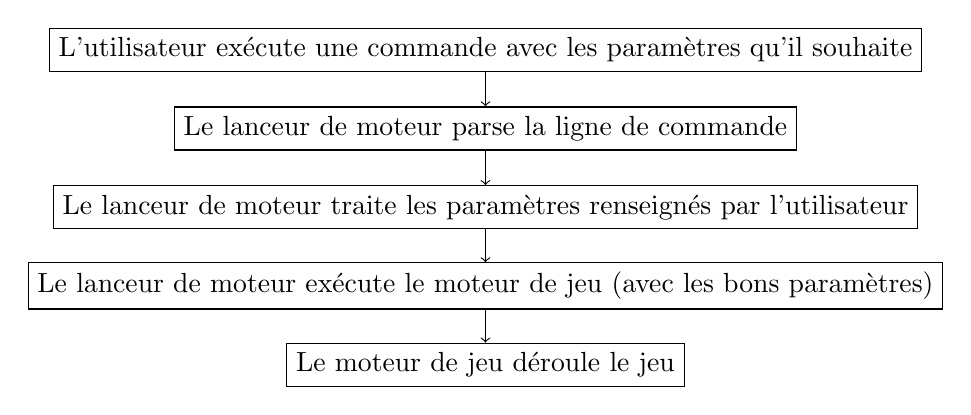
\begin{tikzpicture}
        \node[draw] (user) at (0,0) {L'utilisateur exécute une commande avec les paramètres qu'il souhaite};
        \node[draw] (parse) at (0,-1) {Le lanceur de moteur parse la ligne de commande};
        \node[draw] (param) at (0,-2) {Le lanceur de moteur traite les paramètres renseignés par l'utilisateur};
        \node[draw] (option) at (0,-3) {Le lanceur de moteur exécute le moteur de jeu (avec les bons paramètres)};
        \node[draw] (start) at (0,-4) {Le moteur de jeu déroule le jeu};
        
        \draw[->] (user) -- (parse);
        \draw[->] (parse) -- (param);
        \draw[->] (param) -- (option);
        \draw[->] (option) -- (start);
    \end{tikzpicture}
    
    \caption{Diagramme résumant les étapes d'exécution du logiciel}
    \label{fig:diag_exec}
\end{figure}

\clearpage

\textbf{Résumé du déroulement d'une partie (par le moteur de jeu)}

\begin{figure}[H]
    \centerline{
        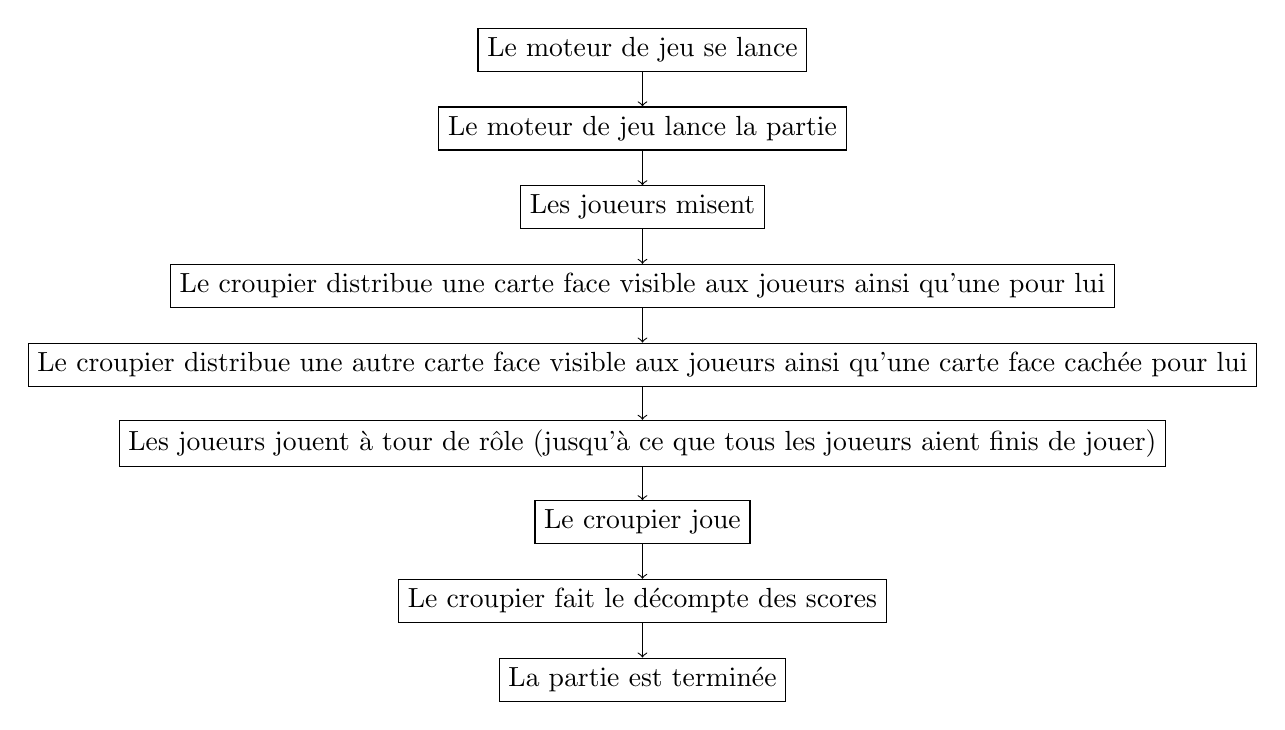
\begin{tikzpicture}[]
            \node[draw] (start1) at (0,0) {Le moteur de jeu se lance};
            \node[draw] (start2) at (0,-1) {Le moteur de jeu lance la partie};
            \node[draw] (bet) at (0,-2) {Les joueurs misent};
            \node[draw] (distrib1) at (0,-3) {Le croupier distribue une carte face visible aux joueurs ainsi qu'une pour lui};
            \node[draw] (distrib2) at (0,-4) {Le croupier distribue une autre carte face visible aux joueurs ainsi qu'une carte face cachée pour lui};
            \node[draw] (play1) at (0,-5) {Les joueurs jouent à tour de rôle (jusqu'à ce que tous les joueurs aient finis de jouer)};
            \node[draw] (play2) at (0,-6) {Le croupier joue};
            \node[draw] (score) at (0,-7) {Le croupier fait le décompte des scores};
            \node[draw] (end) at (0,-8) {La partie est terminée};
            
            \draw[->] (start1) -- (start2);
            \draw[->] (start2) -- (bet);
            \draw[->] (bet) -- (distrib1);
            \draw[->] (distrib1) -- (distrib2);
            \draw[->] (distrib2) -- (play1);
            \draw[->] (play1) -- (play2);
            \draw[->] (play2) -- (score);
            \draw[->] (score) -- (end);
        \end{tikzpicture}
    }

    \caption{Diagramme résumant les étapes d'un déroulement d'une partie avec x joueurs}
    \label{fig:diag_partie}
\end{figure}


\section{Outils utilisés}

Au cours de ce projet, nous avons eu l'occasion d'utiliser divers outils pour des parties précises du développement. 
Pour la réalisation des fichiers \LaTeX, nous avons utilisé l'application web Overleaf, celle-ci nous permettant de travailler à plusieurs facilement et simultanément. De plus, pour la gestion des tâches, nous avons porté notre dévolu sur l'interface web Trello, qui nous a permis de nous répartir aisément le travail tout au long de ce projet grâce à un tableau kanban. 
Pour le développement du code Python, nous avons employé PyCharm en tant qu'IDE et Visual Studio Code en tant qu'éditeur de texte. L'utilisation de ces logiciels a été individuelle et au gré des préférences de chacun. Enfin, nous nous sommes servis de Git et plus particulièrement de GitLab pour collaborer sur le code source et faire de la gestion de version.

\section{Fonctionnement du logiciel}

Dans l'état actuel, le lanceur et le moteur de jeu sont opérationnels et permettent d'effectuer plusieurs parties de 1 à 7 joueurs. Il est aussi possible d'utiliser différents types de joueurs IA, tous les détails pour les utiliser sont disponibles dans la notice d'utilisation du lanceur de moteur ou bien dans le README présent à la racine du projet.

\bigskip

\noindent Voyons ici un exemple simple de fonctionnement de l'application avec 2 parties réalisées par un joueur humain.

\subsection{Lancement du jeu}

Tout d'abord, l'utilisateur doit renseigner les différents arguments qu'il souhaite au lanceur de moteur afin que celui-ci puisse créer le moteur de jeu avec les bonnes valeurs.

\begin{figure}[H]
\begin{minted}
{md}
./run-launcher.sh -j humain -a 1000 -p 2 -d 2 -mn 10 -mx 500 -v

Paramètres de lancement:
  Joueurs : ['Human Player "humain 1":1000']
  Nombre de paquets : 2
  Mises : [10, 500]
  Nombre de parties : 2
  Verbeux : Oui
\end{minted}
\caption{Exemple d'utilisation du lanceur de moteur}
\label{fig:lancement_moteur}
\end{figure} 

Ensuite, la première partie commence et le moteur de jeu demande au joueur la mise qu'il souhaite faire. 

\begin{figure}[H]
\begin{minted}
{md}
humain 1
La mise minimale est : 10
La mise maximale est : 500
Vous avez : 1000
Veuillez entrer la mise que vous souhaitez mettre :
250
\end{minted}
\caption{Exemple de demande de mise pour un joueur humain}
\label{fig:exemple_demande_mise}
\end{figure} 

Lorsque toutes les mises sont renseignées, le moteur de jeu demande aux joueurs la ou les actions qu'ils souhaitent faire. 

\begin{figure}[H]
\begin{minted}
{md}
--------------- Table de jeu ---------------
Joueur "humain 1" :
  5♥ 9♠ (14)
  Mise: 250$
Croupier :
   7♦ ? (7)

humain 1
Veuillez entrer le code de l'action que vous souhaitez faire :
c - Tirer une carte
r - S'arrêter (rester)
d - Doubler sa mise (et recevoir une dernière carte)
a - Abandonner
d
\end{minted}
\caption{Exemple de demande d'action pour un joueur humain}
\label{fig:exemple_demande_action}
\end{figure} 

Une fois que tous les joueurs ont fini de jouer (qu'ils aient abandonné, doublé, brûlé ou qu'ils soient restés), le moteur de jeu fait jouer le croupier. Lorsque celui-ci a fini de jouer, le moteur de jeu calcule et affiche les résultats de la partie.

\begin{figure}[H]
\begin{minted}
{md}
Résultat pour "humain 1" :
  5♥ 9♠ 5♦ (19)
  humain 1 a gagné 500$
  humain 1 a 1500$

Croupier :
  7♦ 2♣ 4♣ 9♣ (22)
\end{minted}
\caption{Exemple d'affichage du résultat d'une partie}
\label{fig:exemple_affichage_resultat_partie}
\end{figure} 

Ensuite, s'il reste encore des parties à jouer et qu'un ou plusieurs joueurs peuvent encore jouer, le moteur de jeu lance la partie suivante.

\begin{figure}[H]
\begin{minted}
{md}
humain 1
La mise minimale est : 10
La mise maximale est : 500
Vous avez : 1500
Veuillez entrer la mise que vous souhaitez mettre :
400

--------------- Table de jeu ---------------
Joueur "humain 1" :
  10♦ K♠ (20)
  Mise: 400$
Croupier :
   9♦ ? (9)

humain 1
Veuillez entrer le code de l'action que vous souhaitez faire :
c - Tirer une carte
r - S'arrêter (rester)
d - Doubler sa mise (et recevoir une dernière carte)
a - Abandonner
r

Résultat pour "humain 1" :
  10♦ K♠ (20)
  humain 1 a gagné 400$
  humain 1 a 1900$

Croupier :
  9♦ 10♠ (19)
\end{minted}
\caption{Exemple complet d'une partie de Blackjack avec un joueur humain}
\label{fig:exemple_partie_complete}
\end{figure} 

Enfin lorsque toutes les parties ont été jouées, le moteur de jeu affiche l'argent de tous les joueurs.

\begin{figure}[H]
\begin{minted}
{md}
Résultat des parties :
  humain 1 a 1900$
\end{minted}
\caption{Exemple d'affichage du résultat final de plusieurs parties}
\label{fig:exemple_affichage_resultat_parties}
\end{figure} 

\newpage

\section{Description des besoins}
Les besoins fonctionnels sont ordonnés par ordre de priorité. En fonction de leur importance, ils sont notés de 1 à 3 (1 étant le niveau avec le plus de priorité). La priorité des besoins est déterminée par rapport à ce que nous jugeons être le plus important dans l'application. \\

Pour certains besoins, nous allons évoquer une machine de spécification minimale, c'est-à-dire, un ordinateur pouvant exécuter l'application avec des composants de puissance minimale. Une machine de spécification minimale doit donc être pourvue à minima de 4Go de mémoire vive, d'un simple processeur basique (ex : dual core 1.7Ghz), de 50Mo d'espace de stockage et ne nécessite pas de GPU.

\subsection{Besoins fonctionnels}

\subsubsection{Le lanceur de moteur de jeu}
\label{sec:launcher}

\begin{enumerate}

    \item \textbf{Analyser les arguments de la ligne de commande :}\\
    Pour connaître les paramètres de la partie, le programme du lanceur de moteur de jeu analyse les arguments et enregistre les valeurs données. Si le nom de l'argument n'est pas reconnu, il est ignoré (ainsi que sa valeur). Une valeur associée à un argument doit avoir une taille inférieure à 100 caractères. Si la valeur d'un argument n'est pas correct, le lanceur doit annoncer l'erreur et arrêter le logiciel. L'utilisateur, joueur ou non de la partie de jeu qui va suivre, décide de la valeur des arguments à fournir (ceci est alors valable et applicable pour les besoins qui suivent concernant les arguments de la ligne de commande). \\
    \textbf{Priorité :} 1. \\
    \textbf{Risques :}
    \begin{itemize}
        \item aucun argument n'est reconnu par le logiciel.
        \item un argument attend une valeur d'un type de donnée précis mais un autre est renseigné.
        \item un argument est trop long en nombre de caractères.
        \item un argument demandant une valeur, mais sans valeur spécifiée.
        \item un argument obligatoire n'est pas renseigné.
    \end{itemize}
    \textbf{Parade :} Afficher un message d'erreur, spécifiant le type d'erreur rencontré.
    
    \item \textbf{Sélectionner le type de joueur (humain/IA) :} \\
    L'argument \code{--joueurs} permet de donner le type ainsi que le nombre des joueurs participants. Les valeurs de ce paramètre peuvent être exprimées par ce regex \code{(<type> <nombre>? )+}. S'il n'y a pas de nombre fourni avec le type, la valeur par défaut, 1 (un), est choisie comme quantité. Une partie peut être lancée uniquement avec des joueurs IA, uniquement des joueurs humains ou les deux.
    Les types possibles sont \code{humain} (pour un joueur humain), \code{ia-basique} (pour une ia appliquant une stratégie basique), \code{ia-hilo} (pour une ia appliquant une stratégie Hi-Lo), \code{ia-hilo-nocount} (pour une ia appliquant une stratégie Hi-Lo sans méthode de comptage) et \code{ia-deep} (pour une ia utilisant le deeplearning). \\
    \textbf{Priorité :} 1. \\
    \textbf{Risques :}
    \begin{itemize}
        \item un type autre que \code{humain}, \code{ia-basique}, \code{ia-hilo}, \code{ia-hilo-nocount} ou \code{ia-deep} est donné.
        \item un nombre négatif est donné.
        \item le nombre total de joueur (humain + IA) est supérieur à 7.
    \end{itemize}
    \textbf{Parade :} Afficher un message d'erreur, spécifiant le type d'erreur rencontré.

    \item \textbf{Lancer un ensemble de parties de jeu :} \\
    Le paramètre \code{--parties <nombre>} permet de définir le nombre de parties que le logiciel va lancer. Le nombre de partie de Blackjack doit être compris entre 0 et 500 inclus.
    Un joueur n'a pas le droit de partir entre plusieurs parties (si le programme est lancé pour 10 parties, chaque joueur devra jouer les 10 parties). Dans le cas où cet argument n'est pas renseigné, le logiciel lancera une seule et unique partie, après laquelle le programme s'arrêtera. Les parties sont lancées consécutivement. Chaque partie se déroule selon les règles du blackjack et les valeurs des arguments passés dans la ligne de commande au départ. \\
    \textbf{Priorité :} 2. \\
    \textbf{Risques :}
    \begin{itemize}
        \item une valeur négative est donnée.
        \item une valeur supérieure à 500 est donnée.
    \end{itemize}
    \textbf{Parade :} Afficher un message d'erreur, spécifiant le type d'erreur rencontré.
    
    \item \textbf{Sélectionner la quantité d'argent de départ par joueur:}\\
    L'argument \code{--argent}, avec comme valeur une liste de nombre détermine la somme d'argent que les joueurs ont au départ de l'exécution. L'ordre de ces nombres correspond à l'ordre des joueurs déterminé par \code{--joueurs}.\\
    Par exemple \code{--joueurs humain 1 ia 2 --argent 10 20 10} se traduit par un joueur humain avec 10 dollars, un joueur IA avec 20 dollars et un joueur IA avec 10 dollars. La somme d'argent de départ d'un joueur doit être comprise entre 0 et 100 000 inclus. \\
    \textbf{Priorité :} 2. \\
    \textbf{Risques :}
    \begin{itemize}
        \item une valeur inférieure à 0 est donnée.
        \item une valeur supérieure à 100 000 est donnée.
        \item le nombre de valeur ne correspond pas au nombre de joueur.
    \end{itemize}
    \textbf{Parade :} Afficher un message d'erreur, spécifiant le type d'erreur rencontré.

    \item \textbf{Sélectionner le nombre de paquet de cartes à utiliser:}\\
    L'option \code{--paquets} détermine le nombre de paquet de cartes que le moteur utilisera durant le jeu. Le nombre de paquet doit être compris entre 1 et 7 inclus. Si il n'y a pas de nombre précisé, la valeur par défaut est 1. \\
    \textbf{Priorité :} 2. \\
    \textbf{Risques :}
    \begin{itemize}
        \item une valeur inférieure à 1 est donnée.
        \item une valeur supérieure à 7 est donnée.
    \end{itemize}
    \textbf{Parade :} Afficher un message d'erreur, spécifiant le type d'erreur rencontré.
    
    \vspace{1cm}
    \begin{figure}[H]
        \includegraphics[width=\textwidth]{{2-besoins/diagramme_renouvellement_paquet.png}}
        \caption{Schéma d'utilisation et renouvellement de plusieurs paquets}
        \label{fig:diag_use_ren_deck}
    \end{figure}
    \vspace{0.5cm}
    
    \item \textbf{Afficher les statistiques d'exécution de l'ensemble des parties :} \\
    Après avoir lancé toutes les parties de Blackjack, le logiciel affiche les statistiques de ces parties de jeu (cf. \hyperref[itm:stats]{Afficher les statistiques liées à un ensemble de partie}). \\
    \textbf{Priorité :} 2. \\
    \textbf{Risques :} aucun. \\
    \textbf{Parade :} aucune.

    \item \textbf{Lire les paramètres du lanceur de moteur de jeu via un fichier:}\\
    Le fichier sera donné via l'argument \code{--fichier params.json}. Si cet argument existe, aucun autre argument n'est pris en compte dans la ligne de commande. C'est le fichier qui dicte les paramètres. Le format des données du fichier est JSON (cf. \nameref{sec:format}). \\
    \textbf{Priorité :} 3. \\
    \textbf{Risques :}
    \begin{itemize}
        \item le format du fichier ne correspond pas à un \code{.json}.
        \item le fichier est corrompu.
        \item les valeurs du fichier ne correspondent pas à des arguments.
        \item les arguments spécifiés ne sont pas complets.
    \end{itemize}
    \textbf{Parade :} Afficher un message d'erreur, spécifiant le type d'erreur rencontré.

    \item \textbf{Sélectionner la mise minimum:}\\
    L'argument \code{--mise-min} détermine la mise minimum par joueur. Cet argument est optionnel. Si il n'est pas renseigné, alors une mise minimum par défaut de 5 dollars est utilisée. La valeur de mise doit être comprise entre 5 et 100 000 inclus. \\
    \textbf{Priorité :} 3. \\
    \textbf{Risques :}
    \begin{itemize}
        \item une valeur inférieure à 5 est donnée.
        \item une valeur supérieure à 100 000 est donnée.
    \end{itemize}
    \textbf{Parade :} Afficher un message d'erreur, spécifiant le type d'erreur rencontré.
    
    \vspace{1cm}
    \begin{figure}[H]
        \includegraphics[width=\textwidth]{{2-besoins/diagramme_utilisation_mise_min.png}}
        \caption{Schéma d'utilisation de la mise minimale par le moteur de jeu pour l'intégration d'un joueur à une partie}
        \label{fig:diag_use_min_bet}
    \end{figure}
    
    \item \textbf{Sélectionner la mise maximum:}\\
    L'argument \code{--mise-max} détermine la mise maximum par joueur. Cet argument est optionnel. Si il n'est pas renseigné alors il n'y a pas de mise maximum (dans la limite où le joueur peut miser une telle quantité). La valeur de mise doit être comprise entre 5 et 100 000 inclus. \\
    \textbf{Priorité :} 3. \\
    \textbf{Risques :}
    \begin{itemize}
        \item une valeur inférieure à 5 est donnée.
        \item une valeur supérieure à 100 000 est donnée.
    \end{itemize}
    \textbf{Parade :} Afficher un message d'erreur, spécifiant le type d'erreur rencontré.

    \item \textbf{Afficher un récapitulatif des paramètres:} \\
    Avant l'exécution des parties, le lanceur de moteur de jeu affichera les paramètres renseignés afin que l'utilisateur puisse voir les paramètres d'exécution. \\
    \textbf{Priorité :} 3. \\
    \textbf{Risques :} aucun. \\
    \textbf{Parade :} aucune.

    \item \textbf{Lancer le programme en exécution rapide:} \\
    Lorsqu'il n'y a que des IA qui jouent, le paramètre \code{--rapide} permet de n'afficher que les résultats de chaque partie (et pas le détail de chaque tour). L'intérêt est de pouvoir exécuter beaucoup de parties rapidement et sans affichage superflu car, par exemple, nous souhaitons tester l'IA ou observer uniquement la finalité de chaque partie de Blackjack.
    Lorsque cet argument est utilisé alors qu'il y a des joueurs humains, il n'a pas d'effet et est ignoré.\\
    \textbf{Priorité :} 3. \\
    \textbf{Risques :} aucun. \\
    \textbf{Parade :} aucune.
 
    \item \textbf{Permettre d'utiliser des raccourcis d'argument:} \\ 
    Chaque argument du logiciel devra avoir une version courte. Par exemple \code{--paquets} aura comme version courte \code{-p}. \\
    \textbf{Priorité :} 3. \\
    \textbf{Risques :} aucun. \\
    \textbf{Parade :} aucune.

\end{enumerate}


\subsubsection{Le moteur de jeu}
\label{sec:engine}

\begin{enumerate}

    \item \textbf{Appliquer les règles du Blackjack:} \\
    Le moteur doit pouvoir réaliser une partie de Blackjack conformément aux règles.
    Le moteur de jeu doit vérifier que les actions faites par les joueurs (IA ou non) sont valides et qu'elles ne viennent donc pas compromettre les règles du jeu. Si le joueur a fait une erreur, le moteur lui redemande. Si au bout de 7 fois le joueur lui répond mal, le moteur élimine le joueur. \\
    \textbf{Priorité :} 1. \\
    \textbf{Risques :} aucun. \\
    \textbf{Parade :} aucune.

    \item \textbf{Afficher l'état du jeu :} \\
    Le moteur doit être capable à chaque tour ou action de joueur d'afficher l'état de jeu et ce qu'il se passe. Il affichera les cartes jouées par chaque joueur (ainsi que le total), les cartes du croupier, les mises, la quantité d'argent totale de chaque joueur, le numéro du tour, l'état du joueur (brulé, en cours, arrété), le paquet utilisé. L'affichage sera textuel et pourra être amélioré en affichage graphique si le temps l'accorde. \\
    \textbf{Priorité :} 1. \\
    \textbf{Risques :} aucun. \\
    \textbf{Parade :} aucune.

    \item \textbf{Afficher les résultats d'une partie:} \\
    A la fin d'une partie, le moteur doit pouvoir afficher le ou les gagnants, les mises gagnées et perdues par joueur, et l'état du jeu. \\
    \textbf{Priorité :} 1. \\
    \textbf{Risques :} aucun. \\
    \textbf{Parade :} aucune.

    \item \textbf{Demander la mise d'un joueur:}\\
    Dans le cas où il y a un joueur humain, le moteur doit être capable au début de chaque partie de jeu de demander la mise d'un joueur en fonction de l'état du jeu. La mise ne sera valide que si le joueur a assez d'argent dans son porte-monnaie. La mise doit être supérieure à la mise minimale spécifiée au lancement de l'application. \\
    \textbf{Priorité :} 1. \\
    \textbf{Risques :} 
    \begin{itemize}
        \item le joueur n'a pas assez d'argent.
        \item une valeur inférieure à la mise minimale est donnée.
    \end{itemize}
    \textbf{Parade :} Afficher un message d'erreur, spécifiant le type d'erreur rencontré.
    
    \item \textbf{Demander une action à un joueur}
    Le moteur doit demander au joueur de lui fournir une action en fonction de l'état du jeu et mettre à jour le jeu en fonction de la-dite action. Tant que le joueur est en jeu, le moteur doit continuer à lui demander une action et mettre à jour le jeu. Si au bout de 7 fois le joueur donne une action incorrecte, il est éliminé de la partie.\\ 
    \textbf{Priorité :} 1. \\
    \textbf{Risque :} 
    \begin{itemize}
        \item une action impossible est donnée par le joueur.
    \end{itemize}
    \textbf{Parade :} Afficher un message d'erreur, spécifiant le type d'erreur rencontré, puis redemander l'action à jouer si le nombre d'essais maximum n'est pas atteint.
    
    \item \textbf{Permettre à plusieurs joueurs de jouer dans une même partie:} \\
    Le moteur de jeu doit être capable de gérer plus d'un joueur dans une même partie.\\
    \textbf{Priorité :} 2.\\
    \textbf{Risques :} 
    \begin{itemize}
        \item le moteur ne peut gérer qu'un seul joueur contre le croupier.
        \item le moteur prend en compte trop de joueur dans la partie.
    \end{itemize}
    \textbf{Parade :} Signaler l'erreur aux développeurs.
    
    \item \textbf{Afficher les statistiques liées à un ensemble de parties :}
    \label{itm:stats}
    \\
    Les statistiques à afficher sont : la carte la plus fréquente, la carte qui gagne le plus souvent, la mise moyenne, la mise la plus petite, la mise la plus grande, les victoires par joueurs, le nombre de tour moyen. \\
    \textbf{Priorité :} 2. \\
    \textbf{Risques :} aucun. \\
    \textbf{Parade :} aucune.
    
\end{enumerate}

\subsubsection{Le joueur humain}
\label{sec:human}

Le joueur humain est le joueur assis devant l'ordinateur qui à chaque fois est interrogé par le moteur au sujet de son action à jouer pour le tour actuel. Dans ce cas, nous prenons l'exemple de l'interface textuelle. Il demandera son action via texte. Il affichera un rappel des actions possibles au blackjack ainsi que le texte à rentrer pour la faire. Si le texte entré par l'utilisateur est valide, il envoie l'action correspondante au moteur, sinon, il redemande à l'utilisateur de saisir un texte en lui expliquant l'erreur qu'il a commise (un certain nombre de fois). 
\begin{enumerate}
    \item \textbf {Miser :} \\
    Il s'agit de l'action liée à la quantité d'argent que le joueur souhaite miser en début de partie. Cette action est demandée en début de partie obligatoirement et ne peut pas être renouvelée par la suite. \\
    \textbf{Priorité :} 2 \\
    \textbf{Risque :} Le joueur entre une valeur de mise supérieure à sa quantité d'argent. \\
    \textbf{Parade :} Afficher un message d'erreur puis redemander la mise au joueur.\\
    \item \textbf {Demander une carte (piocher) :} \\
    Le texte à rentrer pour demander à piocher une carte est \code{carte}, et peut être abrégé par \code{c}. \\
    \textbf{Priorité :} 2 \\
    \textbf{Risque :} Le joueur entre une commande autre que celle spécifiée pour piocher. \\
    \textbf{Parade :} Afficher un message d'erreur puis redemander l'action au joueur.\\
    \item \textbf {Doubler sa mise :} \\
    Le texte à rentrer pour doubler sa mise est \code{double}, et peut être abrégé par \code{d}.
    Il n'est pas possible de piocher par la suite ni de faire une quelconque autre action. \\
    \textbf{Priorité :} 2 \\
    \textbf{Risque :} Le joueur demande de doubler alors qu'il n'a pas la quantité d'argent nécessaire.  \\
    \textbf{Parade :} Afficher un message d'erreur puis redemander une action.\\
    \item \textbf {Se coucher (se retirer) :} \\
    Le texte à rentrer pour se retirer de la partie en cours \code{reste}, et peut être abrégé par \code{r}. Par le biais de cette action le joueur s'arrête de jouer et récupère alors la moitié de sa mise posée au départ. \\
    \textbf{Priorité :} 2 \\
    \textbf{Risque :} Le joueur entre une commande autre que celle spécifiée pour se coucher. \\
    \textbf{Parade :} Afficher un message d'erreur puis redemander une action au joueur.\\
    \item \textbf {Abandonner :} \\
    Le texte à rentrer pour abandonner la partie est \code{abandon}, et peut être abrégé par \code{a}. \\
    \textbf{Priorité :} 2 \\
    \textbf{Risque :} Le joueur entre une commande autre que celle spécifiée pour abandonner. \\
    \textbf{Parade :} Afficher un message d'erreur puis redemander une action au joueur.\\
\end{enumerate}


\subsubsection{Le joueur Intelligence Artificielle}
\label{sec:ia}
\begin{enumerate}
    \item \textbf{Appliquer la stratégie "Basique":} \\
        Le joueur IA doit pouvoir réaliser des actions de jeu conformément aux règles et à la stratégie "Basique", qui correspond à réaliser une certaine action suivant la probabilité de tirer une carte à la valeur avantageuse (cf. \nameref{sec:basic}).
        Cette probabilité est calculée pendant le tour du joueur IA, en comptant les cartes distribuées durant la partie.\\
        \textbf{Priorité :} 1. \\
        \textbf{Risques :} aucun. \\ 
        \textbf{Parade :} aucune.

    \item \textbf{Appliquer la stratégie "Hi-Lo":} \\
        Le joueur IA doit pouvoir réaliser des actions de jeu conformément aux règles et à la stratégie "Hi-Lo", qui fait partie des stratégies les plus simples et populaires du Blackjack (cf. \nameref{sec:hilo}). 
        Elle consiste à assigner une valeur entre -1, 0 et 1 pour chaque carte dans sa main et celle des autres joueurs et du croupier. Nous avons les valeurs suivantes : -1 pour les buches, 0 pour 7, 8 et 9, puis 1 pour les autres cartes. Ainsi il est possible de facilement juger sa main et de la comparer aux autres.\\
        \textbf{Priorité :} 1. \\ 
        \textbf{Risques :} aucun. \\ 
        \textbf{Parade :} aucune.

    \item \textbf{Appliquer la stratégie "Hi-Lo No Count":} \\
        Le joueur IA doit pouvoir réaliser des actions de jeu conformément aux règles et à la stratégie "Hi-Lo No Count" (cf. \nameref{sec:hilonc}). 
        Elle consiste à assigner une valeur entre -1, 0 et 1 pour chaque carte dans sa main. Nous avons les valeurs suivantes : -1 pour les buches, 0 pour 7, 8 et 9, puis 1 pour les autres cartes. Cependant, cette version diffère de la stratégie "Hi-Lo", car elle ne compte pas les cartes apparaissant au cours de la partie.\\
        \textbf{Priorité :} 2. \\ 
        \textbf{Risques :} aucun. \\ 
        \textbf{Parade :} aucune.

    \item \textbf{Appliquer la stratégie "Deep Learning":} \\
        Le joueur IA doit pouvoir réaliser des actions de jeu conformément aux règles du blackajck et à la stratégie "Deep Learning". Celle-ci réalise une certaine action suivant la probabilité de cette dernière, d'après ce que l'IA a appris via les stratégies citées précédemment (cf. \nameref{sec:deep}). Au début de la partie, un réseau de neurones est créé puis entraîné, pour réaliser par la suite les actions qui lui semblent les plus cohérentes lors de son tour. \\
        \textbf{Priorité :} 1. \\
        \textbf{Risques :} aucun. \\ 
        \textbf{Parade :} aucune.
\end{enumerate}

\subsection{Besoins non fonctionnels}

\subsubsection{Besoins Utilisateur}
\begin{enumerate}

    \item \textbf{L'interface du logiciel doit être en français :} \\
    L'interface du programme du jeu doit être compréhensible et écrite en français courant. \\
    \textbf{Priorité :} 1. \\
    \textbf{Risques :} 
    \begin{itemize}
        \item L'affichage et l'interface ne sont pas entièrement en français. \\
    \end{itemize}
    \textbf{Parade :} Signaler l'erreur aux développeurs.
    
    \item \textbf{Le logiciel ne doit avoir accès qu’aux fichiers fournis et pas aux autres disponibles sur la machine :} \\
    \textbf{Priorité :} 1. \\
    \textbf{Risque :} 
    \begin{itemize}
        \item le logiciel accède à des fichiers auxquels il ne devrait pas.
    \end{itemize}
    \textbf{Parade :} Arrêter le chargement du fichier et arrêter le logiciel.
    
     \item \textbf{Le logiciel doit avoir une notice d'utilisation incluse :} \\
    Accessible par une option (comme \code{--help}) si le logiciel est en ligne de commande ou bien un bouton affichant cette notice dans le cas d'un logiciel ayant un affichage graphique. \\
    \textbf{Priorité :} 2. \\
    \textbf{Risques :} aucun. \\
    \textbf{Parade :} aucune.
    
    \item \textbf{Le logiciel doit avoir une version} \\
    Le paramètre \code{--version} affichera la version du logiciel.\\
    \textbf{Priorité :} 3. \\
    \textbf{Risques :} aucun. \\
    \textbf{Parade :} aucune.

\end{enumerate}

\subsubsection{Besoins Système}
\begin{enumerate}
    \item \textbf{Le logiciel doit pouvoir être éxecuté sur GNU/Linux :} \\
    \textbf{Priorité :} 1. \\
    \textbf{Risque(s) :} 
    \begin{itemize}
        \item l’OS ne permet pas d’exécuter le programme.
    \end{itemize}
    \textbf{Parade :} lister les OS et les versions exactes compatibles.
    
    \item \textbf{Le logiciel doit respecter des contraintes de performance :} \\
    \textbf{Priorité :} 1. \\
    \textbf{Risque(s) :} 
    \begin{itemize}
        \item Le lanceur de moteur de jeu doit s'exécuter en moins d'une seconde.
        \item Une IA doit répondre si possible en moins de 10 secondes.
    \end{itemize}
    \textbf{Parade :} Signaler le problème aux développeurs.
\end{enumerate}

\clearpage

\subsection{Diagramme de cas d'utilisation général}

\begin{figure}[H]
    \includegraphics[width=\textwidth]{{2-besoins/diag_cas_util_general_entier.jpg}}
    \caption{Diagramme de cas d’utilisation représentant les principales interactions avec le programme}
    \label{fig:diag_use_case_general}
\end{figure}

\clearpage

\subsection{Description de l'IA}

\subsubsection{Stratégie "Basique"}
\label{sec:basic}

L'IA va déterminer la meilleure action suivant l'état de sa main en évaluant sa valeur. L'algorithme utilisé est probabiliste, c'est-à-dire qu'en fonction des cartes déjà tirées depuis le début de la partie (pour un même paquet), il calcule la probabilité pour chaque carte restante d'être tirée. Si la probabilité d'une carte ayant une valeur intéressante dépasse un certain seuil, précisé en entrée, l'algorithme choisira l'action appropriée. Par exemple, si notre main de départ à une valeur de 11, l'IA va calculer la probabilité de piocher une carte ayant une valeur entre 10 et 6. Ainsi, si cette probabilité est supérieure au seuil haut (ex: 90\%),renvoie l'action "doubler". Cependant, si elle est inférieure au seuil haut mais reste supérieure au seuil bas (ex: 70\%), la probabilité de piocher une bonne carte reste correcte, donc nous renvoyons l'action "piocher".
Ces calculs de probabilité sont effectués seulement si la valeur de la main est inférieure ou égale à une valeur arbitraire. Après une recherche empirique, nous avons estimé que cette valeur serait 17. Ainsi, si la valeur de la main est supérieure, alors l'action renvoyée est "se coucher". De ce fait, ce comportement permet d'éviter sobrement les prises de risque lorsque la main est acceptable.\\
Cet algorithme a une complexité polynomiale en O(m + d), m étant le nombre de cartes dans la main du joueur et d la taille de la collection des cartes comptées (la matrice dynamique md). \\
\\
Algorithme abstrait de la stratégie "Basique" du joueur IA :
\begin{minted}
{md}
Entrées :
main : cartes en main.
p : numéro du paquet.
sh : un seuil haut.
sb : un seuil bas.
argent : la quantité d'argent possédée.
mise : la mise effectuée.

Sortie :
Une action à jouer.

Début.
Pour chaque carte c dans main,
    Ajouter la valeur de c à somme.

Si somme est inférieure ou égale à 17 alors,
    Soustraire somme à 21 et affecter la valeur obtenue à v.

    Pour chaque carte d distribuée ce tour,
        Ajouter à une matrice dynamique md la valeur de d par rapport au paquet p.

    Pour chaque carte c du paquet,
        Si c n’appartient pas à md par rapport au paquet p alors,
            Pour i allant de 0 à 4 inclus,
                Si la valeur de c est égale à la valeur de v - i alors,
                    Incrémenter de 1 t[i].

    max prend la valeur maximum de t.

    Diviser max par la taille de md par rapport au paquet p et affecter la valeur à proba.

    Si proba est supérieure à sh alors,
        Si mise multipliée par 2 est supérieure ou égale à argent alors,
            Retourner l'action Piocher.
        Sinon, 
            Retourner l'action Doubler.
    Si proba est supérieure à sb alors,
        Retourner l'action Piocher.
             
Retourner l'action Arrêter.
Fin.
\end{minted}


\subsubsection{Stratégie "Hi-Lo"}
\label{sec:hilo}

L'IA va déterminer la meilleure action suivant l'état de sa main en évaluant sa valeur, mais également en évaluant la valeur des cartes précédemment distribuée. Cet algorithme diverge de la stratégie "Basique" de part sa manière de compter les cartes. En effet, une carte de valeur 1, 2, 3, 4, 5 ou 6 sera comptée comme une valeur de 1, une carte de valeur 7, 8 ou 9 comme un 0 et une carte de valeur 10 ou 11 comme un -1. Ainsi, en comptant les cartes distribuées avec cette technique, nous pouvons déterminer les valeurs des cartes restantes dans le paquet. Puis en fonction de la valeur de sa main, l'IA peut choisir l'action appropriée. \\
Cet algorithme a une complexité polynomiale en O(m), m étant le nombre de cartes dans la main du joueur. \\
\\
Algorithme abstrait de la stratégie "Hi-Lo" du joueur IA :
\begin{minted}
{md}
Entrées :
main : cartes en main.
p : numéro du paquet.

Sortie :
Une action à jouer.

Début.
Pour chaque carte c dans main,
    Si la valeur de c est égale à 1 ou 2 ou 3 ou 4 ou 5 ou 6 alors,
        ajouter 1 à somme.
    Si la valeur de c est égale à 10 ou 11 alors,
        ajouter -1 à somme.

Diviser somme par la taille de main et affecter la valeur obtenue à u.

Si u est supérieure à 0.5 alors,
    Retourner l'action Piocher.

Si u est inférieure à -0.5 alors,
    Retourner l'action Arrêter.

Pour chaque carte d distribuée ce tour,
    Incrémenter de 1 nombres[p].
    Si la valeur de d est égale à 1 ou 2 ou 3 ou 4 ou 5 ou 6 alors,
       ajouter 1 à sommes[p].
    Si la valeur de d est égale à 10 ou 11 alors,
       ajouter -1 à sommes[p].

Diviser sommes[p] par nombres[p] et affecter la valeur obtenue à v.

Si u est supérieure ou égale à -0.5 et inférieure à 0 et v est supérieure à 0.5, 
ou u est inférieure ou égale à 0.5 et supérieure à 0 et v est inférieure à -0.5 alors,
    Retourner l'action Doubler.

Retourner l'action Arrêter.
Fin.
\end{minted}

\subsubsection{Stratégie "Hi-Lo No Count"}
\label{sec:hilonc}

Cette stratégie se repose sur l'algorithme Hi-Lo développé précédemment. Cependant, cette version d'Hi-Lo ne compte pas les cartes apparaissant au cours de la partie. Ainsi, cette stratégie se concentre uniquement sur la manière de calculer la valeur de la main. Nous attribuons donc les nouvelles valeurs 1, 0 et -1 aux cartes. L'avantage de cette stratégie est qu'elle reste constante sur un ensemble de partie, ce qui permet alors de comparer les résultats avec la stratégie Hi-Lo basée sur le comptage des cartes. \\
Cet algorithme a une complexité polynomiale en O(m), m étant le nombre de cartes dans la main du joueur. \\
\\
Algorithme abstrait de la stratégie "Hi-Lo No Count" du joueur IA :
\begin{minted}
{md}
Entrées :
main : cartes en main.

Sortie :
Une action à jouer.

Début.
Pour chaque carte c dans main,
    Si la valeur de c est égale à 1 ou 2 ou 3 ou 4 ou 5 ou 6 alors,
       ajouter 1 à somme.
    Si la valeur de c est égale à 10 ou 11 alors,
       ajouter -1 à somme.

Diviser somme par la taille de main et affecter la valeur obtenue à u.

Si u est supérieure à 0.5 alors,
    Retourner l'action Piocher.

Retourner l'action Arrêter.
Fin.
\end{minted}

\subsubsection{Algorithme de mise des stratégies "Basique" et "Hi-Lo"}

Cet algorithme de mise est basé sur le comptage de carte et est donc partagé par les stratégies "Basique" et "Hi-Lo". Puisque ces stratégies sont de plus en plus performantes lorsque de plus en plus de cartes sont comptées, les mises effectuées par l'IA se base sur le nombre de cartes comptées. Sur un ensemble de partie, les mises réalisées seront donc progressivement plus importantes. L'algorithme se base également sur la somme actuelle d'argent possédée par l'IA. Cela permet de garantir que l'IA misera une somme en accord avec ce qu'elle possède et donc éviter des mises impossibles. \\
Cet algorithme a une complexité polynomiale en O(1). \\
\\
Algorithme abstrait de mise des joueurs IA "Basique" et "Hi-Lo" :
\begin{minted}
{md}
Entrées :
p : numéro du paquet.
argent : la quantité d'argent possédée.
misemin : mise minimale acceptée.
misemax : mise maximale acceptée.

Sortie :
Une valeur à miser.

Début.
mise prend la valeur misemin.

Si le nombre de cartes comptées pour le paquet p est supérieur à 0 alors,
    Multiplier argent par le nombre de carte comptée et affecter la valeur obtenue à m.
    Diviser m par la taille d'un paquet complet et affecter la valeur obtenue à mise.
    
    Si mise est inférieure à misemin alors,
        mise prend la valeur misemin.
        
    Si mise est supérieure à misemax alors,
        mise prend la valeur misemax.

Retourner mise.
Fin.
\end{minted}

\subsubsection{Stratégie Deep Learning}
\label{sec:deep}

\paragraph{Explication générale}
Cette intelligence artificielle est fortement basée sur les stratégies "Basique" et "Hi-Lo". En effet, comme son nom l'indique, elle s'appuie sur un réseau de neurones artificiel, qui permettent à l'IA d'apprendre. Pour se faire, il faut ce que nous appelons un ensemble de données (dataset) à fournir à notre réseau. Nous avons crée nos propres données regroupées sous la forme d'un fichier CSV. Ce fichier CSV contient donc un ensemble de partie, et pour chacune d'entre elles, nous savons quel type d'IA a joué, si elle a gagné, les cartes qu'elle avait, ainsi que les cartes que possédait le croupier. Ci-dessous, un extrait du format du fichier qui est utilisé. \\

\begin{figure}[H]
    \csvautotabular{2-besoins/dataset_exemple.csv} 
    \caption{Extrait du fichier CSV utilisé pour créer le dataset}
    \label{fig:csv_exemple}
\end{figure}

Cependant, le fichier n'est pas utilisé tel quel. Il faut formater les données, mais aussi choisir uniquement les informations que nous considérons essentielles au bon fonctionnement du réseau de neurones, et un temps de calcul raisonnable. Pour cela, nous considérons uniquement deux dimensions, qui sont la somme des cartes du joueur (ici c'est une IA développée précédemment), ainsi que la première carte du croupier car au moment de la partie, nous ne connaissons qu'une seule carte du croupier, celle face visible. Nous avons donc en entrée un vecteur de taille 2, qui va être traité par le réseau de neurones, et en sortie nous avons un vecteur de taille 4. Chaque élément de ce vecteur de sortie est exprimé sous la forme d'une probabilité et se réfère donc à une action possible lors de la partie. Le premier élément correspond à l'action de piocher, le second à l'action de rester, le troisième à l'action de doubler et enfin le dernier à l'action d'abandonner. Lors d'une partie, l'IA basée sur le deeplearning est capable de retourner l'action avec la plus haute probabilité selon ce qu'elle a appris, dans notre cas, via le fichier CSV construit au cours des parties. 

\paragraph{Réseau de neurones}
Notre réseau de neurones est constitué d'une couche d'aplatissement en entrée, de 3 couches cachées intermédiaires, et d'une couche de sortie dite softmax, qui permet d'attribuer une probabilité à chaque action selon le vecteur en entrée. 
Les trois couches cachées sont toutes de types dense, la première comporte 128 neurones, la seconde 64 et la troisième 32. Chaque couche a pour fonction d'activation la fonction ReLU qui choisi le maximum entre x (la valeur fournie) et 0. Cette fonction a été choisie car nous avons ici une classification non-binaire (plusieurs actions possibles à la fin et non uniquement deux), mais aussi car c'est une des fonctions les plus performantes et utilisées pour les couches denses dans de tels réseaux de neurones. \\
Pour la couche de sortie, il s'agit d'une couche dense de taille 4 (représentant le nombre de classes, soit le nombre d'actions possibles lors d'une partie), utilisant la fonction d'activation softmax. Comme précisé auparavant, cette couche permet de transformer notre vecteur d'entiers, en vecteurs de probabilités. C'est la fonction que nous avons choisi car elle est parfaitement adaptée aux problèmes multi-classes, comme c'est le cas ici. Nous avons ainsi une probabilité pour chaque action. 
\begin{figure}[H]
    \includegraphics[width=\textwidth]{{2-besoins/reseau_neurones.png}}
    \caption{Schéma du réseau de neurones implémenté}
    \label{fig:reseau_neurones}
\end{figure} 

Enfin, lors de la compilation du modèle, il est important de choisir la bonne fonction de perte. Dans notre cas, la meilleure fonction minimisant la perte est celle calculant la moyenne des carrés des erreurs entre la vérité terrain et la prédiction. Ensuite, lors de l'entraînement du modèle, la taille des "batchs" ainsi que le nombre "d'épochs" est important. Nous avons choisi un nombre d'épochs de 256, car il faut que celui-ci soit suffisamment important lorsque la taille du dataset est considérable, ce qui est le cas. Néanmoins, il ne doit pas non plus être trop grand pour éviter le phénomène d'overfitting, ce qui pousserait notre modèle à trop se coller au set d'entraînement et donc de fournir des prédictions plutôt mauvaises. 
Pour le nombre de batchs, 64 suffit amplement, sans être trop important, également pour suivre le même raisonnement que donné juste avant. Enfin notre dataset est quant à lui partagé en deux, une partie pour l'entraînement et une partie pour tester le modèle. Nous avons choisi de donner 85\% pour l'entraînement et le reste pour les tests. Avec l'ensemble de ces paramètres nous avons un modèle avec un taux de précision aux alentours de 72\% et une perte autour de 0.1 (varie entre 0.09 et 0.1).  
\begin{figure}[H]
    \includegraphics[width=\textwidth]{{2-besoins/acc_plot.pdf}}
    \caption{Précision du modèle au cours de l'apprentissage}
    \label{fig:plot_acc_modele}
\end{figure} 

\begin{figure}[H]
    \includegraphics[width=\textwidth]{{2-besoins/loss_plot.pdf}}
    \caption{Fonction de perte du modèle au cours de l'apprentissage}
    \label{fig:plot_loss_modele}
\end{figure} 

\paragraph{Recherches des paramètres}

Afin d'atteindre de tels résultats, il a fallu passer par des périodes de recherches pour trouver des bons paramètres. Au départ, notre vecteur en entrée était de taille 6, puis nous avons vu que certains critères n'influençaient pas sur la prédiction, donc les retirer était plus pertinent. Ensuite, la répartition des données entre apprentissage et test était respectivement de 70\% et 30\%, donc nous avons favorisé l'apprentissage en donnant 85\% des données. Une légère augmentation de la précision du modèle a pu être observée via la modification de ces deux paramètres (de 65\% à 69\%). \\
Nous nous sommes alors dirigés ensuite sur le nombre de couches cachées et leurs tailles. En ajouter ne procurait aucune amélioration de la précision. Quant à la taille des épochs et des batchs, les augmenter a permis d'avoir une meilleure précision (autour de 70\%), mais la perte pendant ce temps restait toujours très élevée (environ 0.8). Il a fallu simplement changer la fonction de perte qui était de base "cross entropy" en "mean squared error". Nous avons eu une descente de la perte aux alentours de 0.1. La cross entropy pouvait sembler correspondre, or le problème est qu'elle ne sert qu'à calculer des différences entre des probabilités. Pour notre vérité terrain, une probabilité est au maximum et les autres à zéro ce qui augmente la perte. C'est pourquoi la moyenne des carrés des erreurs est plus favorable dans notre cas, avec l'utilisation de probabilités comme nous l'avons fait pour la vérité terrain et les prédictions. 


\newpage

\section{Architecture du logiciel}
Pour créer ce logiciel, nous avons utilisé le langage Python. La raison première de ce choix est l'utilisation de Keras et Tensorflow, des bibliothèques de deeplearning. 

\subsection{Une décomposition modulaire du code}

Grâce à une programmation orientée objet, nous avons pu concevoir le logiciel de telle sorte à ce qu'il y ai plusieurs modules interchangeables. Nous avons ainsi trois modules principaux : le moteur, le lanceur et les joueurs. Le moteur permet d'exécuter plusieurs parties de blackjack. Le lanceur permet de configurer le moteur selon les désirs de l'utilisateur et de le démarrer, c'est le point d'entrée du programme. Les joueurs fournissent des implémentations différentes pour chaque algorithme.

Nous avons créé le moteur de telle sorte qu'il soit totalement hermétique à l'implémentation d'un joueur et de la manière dont le moteur est utilisé. De plus, nous avons rendu le moteur très configurable dans son exécution. C'est-à-dire que le moteur seulement n'est pas capable de lancer des parties de blackjack et d'y jouer. Nous avons conçu le moteur comme une bibliothèque qui a besoin d'un code client pour exploiter tout son potentiel. C'est celui-ci qui viendra définir les paramètres d'exécution ainsi que les différentes implémentations de joueurs.
En effet, le moteur se base sur l'abstraction d'un joueur. Cette abstraction nous a permis plus tard de pouvoir réaliser différents joueurs qui ont chacun un algorithme différent sans changer le code du moteur. Nous nous sommes servis de la programmation objet et du principe de substitution de Liskov ainsi que de l'inversion de dépendances pour faire cela.

Le lanceur est le module qui sert d'entrée du programme. C'est celui-ci qui va paramétrer le moteur, lui fournir les joueurs et lancer la partie. Le lanceur que nous avons fait est en ligne de commande et utilise les arguments définis par l'utilisateur pour paramétrer le moteur.

Le module joueur fourni les différentes implémentations de joueur. Nous avons créé un joueur par algorithme. Les algorithmes étant "Basique", "Hi-Lo", "Hi-Lo No Count", "Deep Learning" et humain (bien qu'il n'y ai pas réellement d'algorithme).

Nous avons un quatrième module pour gérer l'affichage des données et du jeu. De même que pour les joueurs, le moteur se sert d'une abstraction de l'affichage pour permettre d'avoir plusieurs types d'affichages possibles sans modification du code du moteur. Nous avons créé une implémentation de l'affichage qui est en mode textuel dans un terminal.

\subsection{Diagramme de classes}

La page ci-dessous présente le diagramme de classes simplifié représentant les interactions entre les classes de l'application. Celui-ci ne contient pas les attributs et méthodes des différentes classes. C'est pourquoi, une \hyperref[subsec:class-diagram]{version complète du diagramme de classe}  se trouve en annexe.

\includepdf[landscape=true]{3-architecture/simplified_class_diagram.pdf}

\begin{figure}[H]
\caption{Diagramme de classes simplifié représentant les interactions entre les classes de l'application}
\label{fig:simplified_class_diagram}
\end{figure}

\subsection{Bibliothèques externes utilisées}

Pour développer l'implémentation d'un joueur se basant sur le deeplearning, nous nous sommes servis des bibliothèques TensorFlow \cite{ref-tensorflow}, Keras \cite{ref-keras}, NumPy \cite{ref-numpy} et Pandas\cite{ref-pandas}. TensorFlow et Keras sont des bibliothèques permettant de faire des calculs de deeplearning. NumPy sert à faire des calculs mathématiques et est utilisée par TensorFlow. Pandas sert à manipuler facilement les données d'un fichier CSV. Sans ces bibliothèques, il nous aurait été impossible de produire une IA basée sur du deeplearning.

De plus, nous avons utilisé deux fonctions utilitaires dans le moteur que nous avons trouvé sur StackOverflow. Le lien vers la page est renseigné au niveau de la documentation du code.

\subsection{Implémentation du jeu}

Pour implémenter l'exécution d'une partie de jeu et faire en sorte que les joueurs aient toutes les données du plateau de jeu à chaque instant, nous avons mis en place plusieurs évènements afin de donner aux joueurs les nouvelles informations.

Il y a deux évènements, le début de la partie et sa fin, qui sont obligatoires et lancés à chaque partie. Il est assuré qu'ils ne sont lancés qu'une seule fois par partie.

Les autres évènements sont optionnels et multiples. C'est-à-dire qu'un de ceux-ci peut ne pas être lancé durant une partie, comme il peut être lancé plusieurs fois. Ces évènements sont "gain d'une nouvelle carte", "un autre joueur a gagné une carte", "le croupier a gagné une carte", et "la défausse a été remise dans la pioche".

Ainsi, au début de la partie, le moteur va notifier les joueurs du début de la partie, puis demander leur mise. Une fois les mises définies, le moteur notifie les joueurs de leurs cartes, de celles de leurs camarades et celle visible du croupier. Ensuite, pour chaque joueur le moteur demande les actions que le joueur décide de faire et notifie les joueurs du résultat de l'action. Une fois que chaque joueur a terminé toutes ses actions, le moteur notifie le joueur des cartes piochées par le croupier puis les notifie de la fin de la partie.

\begin{figure}[H]
    \begin{tikzpicture}
    \begin{umlseqdiag}
        \umlobject{Engine}
        \umlobject{Player1}
        \umlobject{Player2}
        \begin{umlcall}[op={notify\_game\_start()}]{Engine}{Player1}
        \begin{umlcall}[op={notify\_game\_start()}]{Engine}{Player2}
        \begin{umlcall}[op={get\_bet()}, return=value]{Engine}{Player1}
        \end{umlcall}
        \begin{umlcall}[op={get\_bet()}, return=value]{Engine}{Player2}
        \end{umlcall}
        \begin{umlcall}[op={notify\_new\_card()}]{Engine}{Player1}
        \end{umlcall}
        \begin{umlcall}[op={notify\_new\_bud\_card()}]{Engine}{Player2}
        \end{umlcall}
        \begin{umlcall}[op={notify\_new\_card()}]{Engine}{Player2}
        \end{umlcall}
        \begin{umlcall}[op={notify\_new\_bud\_card()}]{Engine}{Player1}
        \end{umlcall}
        \begin{umlcall}[op={notify\_new\_dealer\_card()}]{Engine}{Player1}
        \end{umlcall}
        \begin{umlcall}[op={notify\_new\_dealer\_card()}]{Engine}{Player2}
        \end{umlcall}
        \begin{umlcall}[op={notify\_new\_card()}]{Engine}{Player1}
        \end{umlcall}
        \begin{umlcall}[op={notify\_new\_bud\_card()}]{Engine}{Player2}
        \end{umlcall}
        \begin{umlcall}[op={notify\_new\_card()}]{Engine}{Player2}
        \end{umlcall}
        \begin{umlcall}[op={notify\_new\_bud\_card()}]{Engine}{Player1}
        \end{umlcall}
        \begin{umlfragment}[type=loop, name=play1]
            \begin{umlcall}[op={next\_action()}, return=action]{Engine}{Player1}
            \end{umlcall}
        \end{umlfragment}
        \umlnote[x=-4, y=-12]{play1}{tant que Player1 peut jouer}
        \begin{umlfragment}[type=loop, name=play2]
            \begin{umlcall}[op={next\_action()}, return=action]{Engine}{Player2}
            \end{umlcall}
        \end{umlfragment}
        \umlnote[x=-4, y=-14]{play2}{tant que Player2 peut jouer}
        \begin{umlcall}[op={notify\_game\_end()}]{Engine}{Player1}
        \end{umlcall}
        \begin{umlcall}[op={notify\_game\_end()}]{Engine}{Player2}
        \end{umlcall}
        \end{umlcall}
        \end{umlcall}
    \end{umlseqdiag}
    \end{tikzpicture}
    \caption{Diagramme de séquence décrivant le déroulement simplifié d'une partie.}
\end{figure}


\newpage

\section{Analyse du logiciel et tests}
\subsection{Analyse des performances du logiciel}
L'état actuel des stratégies nous permet de déduire des résultats que nous conservons dans un ensemble de données utilisé par le réseau de neurones pour s'entraîner. À partir de ces données, nous avons pu déduire une moyenne de réussite pour chaque stratégie (sauf Deep Learning qui a déjà été présenté précédemment): environ 40\% pour la stratégie "Basique", 38\% pour la stratégie "Hi-Lo" et enfin 37\% pour "Hi-Lo No Count". Nous considérons comme réussite uniquement les cas où le joueur intelligence artificielle gagne la partie. Cependant, si nous considérons également les égalités comme cas de victoire, toutes les moyennes de réussite augmentent environ de 7\%. Ces chiffres nous permettent de nous rendre compte que des améliorations sont encore possibles. De plus, nous pouvons aussi optimiser ces résultats en modifiant les paramètres d'entrées des algorithmes de décision des stratégies. Dans la dernière version de l'application, les paramètres important de la stratégie "Basique" sont le seuil bas qui est à 0.08 et le seuil haut qui vaut 0.5. Ces valeurs ont été choisi empiriquement à la suite de plusieurs tests manuels et d'observations sur les probabilités calculées.

\subsection{Présentation du développement des tests}
Dans le but de vérifier le bon fonctionnement de notre logiciel nous avons effectué plusieurs tests à différentes échelles de l'application. Nous avons utilisé des tests unitaires pour la vérification des résultats des méthodes de classe utilisées par le moteur de jeu et les différents types de joueurs, en fonction des entrées des méthodes. Le déroulement de la partie, comprenant la bonne application des règles du Blackjack et le bon comportement de l'intelligence artificielle, ont été vérifiés majoritairement par de multiples tests "manuels" qui consistait à lancer le logiciel sur une partie type, en utilisant des joueurs "humains" pour en modifier les scénarios à un instant donné du jeu. Ce choix de tests "manuels" a été amené par la difficulté de pré-programmer efficacement l'ensemble des parties décrivant tous les scénarios possibles de ce jeu à information partielle et donc à nature probabiliste.

\subsection{Tests des besoins fonctionnels}

\subsubsection{Le lanceur de moteur de jeu}

\begin{enumerate}
    \item \textbf{Analyser les arguments de la ligne de commande :}
    \begin{itemize}
        \item \textbf{Données :} une machine de spécification minimale, l'application développée, une ligne de commande.
        \item \textbf{Résultats attendus :} 
        \begin{itemize}
            \item positif: l'application se lance correctement. \item négatif: un message d'erreur est affiché.
        \end{itemize}
        \item \textbf{Scénario positif :}
        \begin{itemize}
            \item L’utilisateur ouvre un terminal.
            \item L’utilisateur entre une commande avec des arguments valides.
            \item L'application se lance correctement en prenant en compte les arguments.
        \end{itemize}
        \item \textbf{Scénario négatif :}
        \begin{itemize}
            \item L’utilisateur ouvre un terminal.
            \item L’utilisateur entre une commande avec des arguments invalides.
            \item Un message d'erreur apparaît.
        \end{itemize}
    \end{itemize}
    
    \item \textbf{Sélectionner le type de joueur (humain/IA) :}
    \begin{itemize}
        \item \textbf{Données :} une machine de spécification minimale, l'application développée, une ligne de commande.
        \item \textbf{Résultats attendus :}
        \begin{itemize}
            \item positif: l'application se lance correctement. \item négatif: un message d'erreur est affiché.
        \end{itemize}
        \item \textbf{Scénario positif:}
        \begin{itemize}
            \item L’utilisateur ouvre un terminal.
            \item L’utilisateur entre la commande avec l'argument \code{--joueurs (ia 5? )+}.
            \item L'application se lance correctement avec 5 joueurs IA.
        \end{itemize}
        \item \textbf{Scénario négatif:}
        \begin{itemize}
            \item L’utilisateur ouvre un terminal.
            \item L’utilisateur entre la commande avec l'argument \code{--joueurs (humain 16? )+}.
            \item Un message d'erreur apparaît.
        \end{itemize}
    \end{itemize}

    \item \textbf{Lancer un ensemble de parties de jeu :}
    \begin{itemize}
        \item \textbf{Données :} une machine de spécification minimale, l'application développée, une ligne de commande.
        \item \textbf{Résultats attendus :}
        \begin{itemize}
            \item positif: l'application se lance correctement. \item négatif: un message d'erreur est affiché.
        \end{itemize}
        \item \textbf{Scénario positif :}
        \begin{itemize}
            \item L’utilisateur ouvre un terminal.
            \item L’utilisateur entre la commande avec l'argument \code{--parties 25}.
            \item L'application se lance correctement et va exécuter 25 parties.
        \end{itemize}
        \item \textbf{Scénario négatif :}
        \begin{itemize}
            \item L’utilisateur ouvre un terminal.
            \item L’utilisateur entre la commande avec l'argument \code{--parties -7}.
            \item Un message d'erreur apparaît.
        \end{itemize}
    \end{itemize}
    
    \item \textbf{Sélectionner la quantité d'argent de départ par joueur:}
    \begin{itemize}
        \item \textbf{Données :} une machine de spécification minimale, l'application développée, une ligne de commande.
        \item \textbf{Résultats attendus :} 
        \begin{itemize}
            \item positif: l'application se lance correctement. \item négatif: un message d'erreur est affiché.
        \end{itemize}
        \item \textbf{Scénario positif :}
        \begin{itemize}
            \item L’utilisateur ouvre un terminal.
            \item L’utilisateur entre la commande avec l'argument \code{--argent 4000 500 6000}.
            \item L'application se lance correctement avec les sommes spécifiées.
        \end{itemize}
        \item \textbf{Scénario négatif :}
        \begin{itemize}
            \item L’utilisateur ouvre un terminal.
            \item L’utilisateur entre la commande avec l'argument \code{--argent 9999999 -3 6000}.
            \item Un message d'erreur apparaît.
        \end{itemize}
    \end{itemize}

    \item \textbf{Sélectionner le nombre de paquet de cartes à utiliser:}
    \begin{itemize}
        \item \textbf{Données :} une machine de spécification minimale, l'application développée, une ligne de commande.
        \item \textbf{Résultats attendus :} 
        \begin{itemize}
            \item positif: l'application se lance correctement. \item négatif: un message d'erreur est affiché.
        \end{itemize}
        \item \textbf{Scénario positif :}
        \begin{itemize}
            \item L’utilisateur ouvre un terminal.
            \item L’utilisateur entre la commande avec l'argument \code{--paquets 3}.
            \item L'application se lance et prépare 3 paquets de cartes.
        \end{itemize}
        \item \textbf{Scénario négatif :}
        \begin{itemize}
            \item L’utilisateur ouvre un terminal.
            \item L’utilisateur entre la commande avec l'argument \code{--paquets 8}.
            \item Un message d'erreur apparaît.
        \end{itemize}
    \end{itemize}

    \item \textbf{Afficher les statistique d'exécution de l'ensemble des parties :} \\
    Aucun test n'a été implémenté pour ce cas.

    \item \textbf{Lire les paramètres du lanceur de moteur de jeu via un fichier:}
    \begin{itemize}
        \item \textbf{Données :} une machine de spécification minimale, l'application développée, une ligne de commande, un fichier JSON, un fichier HTML.
        \item \textbf{Résultats attendus :} 
        \begin{itemize}
            \item positif: l'application se lance correctement. \item négatif: un message d'erreur est affiché.
        \end{itemize}
        \item \textbf{Scénario positif :}
        \begin{itemize}
            \item L’utilisateur ouvre un terminal.
            \item L’utilisateur entre la commande avec l'argument \code{--fichier params.json}.
            \item L'application se lance correctement et lit bien les arguments depuis le fichier JSON.
        \end{itemize}
        \item \textbf{Scénario négatif :}
        \begin{itemize}
            \item L’utilisateur ouvre un terminal.
            \item L’utilisateur entre la commande avec l'argument \code{--fichier params.html}.
            \item Un message d'erreur apparaît.
        \end{itemize}
    \end{itemize}

    \item \textbf{Sélectionner la mise minimum:}
    \begin{itemize}
        \item \textbf{Données :} une machine de spécification minimale, l'application développée, une ligne de commande.
        \item \textbf{Résultats attendus :} 
        \begin{itemize}
            \item positif: l'application se lance correctement. \item négatif: un message d'erreur est affiché.
        \end{itemize}
        \item \textbf{Scénario positif :}
        \begin{itemize}
            \item L’utilisateur ouvre un terminal.
            \item L’utilisateur entre la commande \code{--mise-min 20}.
            \item L'application se lance correctement avec une mise minimale de 20 dollars.
        \end{itemize}
        \item \textbf{Scénario négatif :}
        \begin{itemize}
            \item L’utilisateur ouvre un terminal.
            \item L’utilisateur entre la commande \code{--mise-min 3}.
            \item Un message d'erreur apparaît.
        \end{itemize}
    \end{itemize}

    \item \textbf{Sélectionner la mise maximum:}
    \begin{itemize}
        \item \textbf{Données :} une machine de spécification minimale, l'application développée, une ligne de commande.
        \item \textbf{Résultats attendus :} 
        \begin{itemize}
            \item positif: l'application se lance correctement. \item négatif: un message d'erreur est affiché.
        \end{itemize}
        \item \textbf{Scénario positif :}
        \begin{itemize}
            \item L’utilisateur ouvre un terminal.
            \item L’utilisateur entre la commande \code{--mise-max 1000}.
            \item L'application se lance correctement avec une mise maximale de 1 000 dollars.
        \end{itemize}
        \item \textbf{Scénario négatif :}
        \begin{itemize}
            \item L’utilisateur ouvre un terminal.
            \item L’utilisateur entre la commande \code{--mise-max 2}.
            \item Un message d'erreur apparaît.
        \end{itemize}
    \end{itemize}

    \item \textbf{Afficher un récapitulatif des paramètres:}\\
    Aucun test n'a été implémenté pour ce cas.

    \item \textbf{Lancer le programme en exécution rapide:} \\
    Aucun test n'a été implémenté pour ce cas.

    \item \textbf{Permettre d'utiliser des raccourcis d'argument:}  \\
    Aucun test n'a été implémenté pour ce cas.

\end{enumerate}

\subsubsection{Le moteur de jeu}

\begin{enumerate}
    \item \textbf{Appliquer les règles du Blackjack:} \\
    Aucun test n'a été implémenté pour ce cas.

    \item \textbf{Afficher l'état du jeu :} \\
    Aucun test n'a été implémenté pour ce cas.

    \item \textbf{Afficher les résultats d'une partie:} \\
    Aucun test n'a été implémenté pour ce cas.

    \item \textbf{Demander la mise d'un joueur:}
    \begin{itemize}
        \item \textbf{Données :} une machine de spécification minimale, l'application développée, une ligne de commande.
        \item \textbf{Résultats attendus :}
        \begin{itemize}
            \item positif: la mise proposée est acceptée. 
            \item négatif: un message d'erreur est affiché.
        \end{itemize}
        \item \textbf{Scénario positif :}
        \begin{itemize}
            \item L'utilisateur lance l'application avec une ligne de commande.
            \item L'application demande à l'utilisateur combien il veut miser.
            \item L'utilisateur mise 50 dollars alors qu'il lui en reste 457.
            \item L'application accepte la mise du joueur.
        \end{itemize}
        \item \textbf{Scénario négatif :}
        \begin{itemize}
            \item L'utilisateur lance l'application avec une ligne de commande.
            \item L'application demande à l'utilisateur combien il veut miser.
            \item L'utilisateur mise 50 dollars alors qu'il lui en reste 23.
            \item Un message d'erreur apparaît.
            \item L'application redemande à l'utilisateur.
        \end{itemize}
    \end{itemize}

    \item \textbf{Demander une action à un joueur}
    \begin{itemize}
        \item \textbf{Données :} une machine de spécification minimale, l'application développée, une ligne de commande.
        \item \textbf{Résultats attendus :}
        \begin{itemize}
            \item positif: l'action proposée est acceptée.
            \item négatif: un message d'erreur est affiché.
        \end{itemize}
        \item \textbf{Scénario positif :}
        \begin{itemize}
            \item L'utilisateur lance l'application avec une ligne de commande.
            \item L'application demande au joueur quelle action il veut réaliser.
            \item Le joueur entre une action possible.
            \item L'application accepte l'action entrée par le joueur.
        \end{itemize}
        \item \textbf{Scénario négatif :}
        \begin{itemize}
            \item L'utilisateur lance l'application avec une ligne de commande.
            \item L'application demande au joueur quelle action il veut réaliser.
            \item Le joueur entre une action impossible.
            \item Un message d'erreur apparaît.
            \item L'application redemande une action au joueur.
        \end{itemize}
    \end{itemize}

    \item \textbf{Permettre à plusieurs joueurs de jouer dans une même partie:}
    \begin{itemize}
        \item \textbf{Données :} une machine de spécification minimale, l'application développée, une ligne de commande.
        \item \textbf{Résultats attendus :} 
        \begin{itemize}
            \item positif: l'application exécute la partie correctement.
            \item négatif: l'application s'arrête.
        \end{itemize}
        \item \textbf{Scénario positif :}
        \begin{itemize}
            \item L'utilisateur lance l'application avec une ligne de commande en spécifiant 2 joueurs.
            \item L'application gère les deux joueurs.
            \item L'application continue de fonctionner normalement.
        \end{itemize}
        \item \textbf{Scénario négatif :}
        \begin{itemize}
            \item L'utilisateur lance l'application avec une ligne de commande en spécifiant 2 joueurs.
            \item L'application n'arrive pas à gérer les deux joueurs.
            \item L'application s'arrête.
        \end{itemize}
    \end{itemize}
    
    \item \textbf{Afficher les statistiques liées à un ensemble de parties :}\\
    Aucun test n'a été implémenté pour ce cas.
    
\end{enumerate}

\subsubsection{Le joueur humain}

\begin{itemize}
    \item \textbf{Données :} une machine de spécification minimale, l'application développée, une ligne de commande.
    \item \textbf{Résultats attendus :} 
        \begin{itemize}
            \item positif: l'application s'exécute correctement. \item négatif: un message d'erreur est affiché.
        \end{itemize}
    \item \textbf{Scénario positif :}
    \begin{itemize}
        \item L'utilisateur lance l'application avec une ligne de commande.
        \item L'application demande au joueur quelle action il veut réaliser.
        \item Le joueur entre l'action \code{piocher}.
        \item L'action est reconnue et l'application continue de fonctionner normalement.
    \end{itemize}
    \item \textbf{Scénario négatif :}
    \begin{itemize}
        \item L'utilisateur lance l'application avec une ligne de commande.
        \item L'application demande au joueur quelle action il veut réaliser.
        \item Le joueur entre l'action \code{jeter}.
        \item L'action n'est pas reconnue et un message d'erreur apparaît.
    \end{itemize}
\end{itemize}

\subsubsection{Le joueur Intelligence Artificielle}

\begin{enumerate}
    \item \textbf{Appliquer la stratégie "Basique":} 
    \begin{enumerate}
        \item Renvoyer l'action "Piocher"
        \begin{itemize}
            \item \textbf{Données :} une machine de spécification minimale, l'application développée.
            \item \textbf{Résultat attendue :} L'intelligence artificielle renvoie l'action attendue qui est "Piocher".
            \item \textbf{Scénario du test :}
            \begin{itemize}
                \item Une nouvelle partie commence.
                \item Le croupier pioche un six de coeur et une carte cachée.
                \item Le joueur IA pioche un dix de carreaux et un quatre de coeur.
                \item Le joueur IA décide d'une action.
            \end{itemize}
            
            \item \textbf{Résultat concret : } Ce test est validé. La probabilité de piocher une carte intéressante (d'après la stratégie) dans ce cas est de 0.082 et le seuil bas (celui que nous cherchons à atteindre) est de 0.08.
        \end{itemize}

        \item Renvoyer l'action "Doubler"
        \begin{itemize}
            \item \textbf{Données :} une machine de spécification minimale, l'application développée.
            \item \textbf{Résultat attendue :} L'intelligence artificielle renvoie l'action attendue qui est "Doubler".
            \item \textbf{Scénario du test :}
            \begin{itemize}
                \item Plusieurs parties se déroulent et le joueur IA compte les cartes.
                \item Une nouvelle partie commence.
                \item Le croupier pioche un neuf de coeur et une carte cachée.
                \item Le joueur IA pioche un trois de carreau et un Roi de coeur.
                \item Le joueur IA décide d'une action.
            \end{itemize}
            
            \item \textbf{Résultat concret : } Ce test est validé. La probabilité de piocher une carte intéressante (d'après la stratégie) dans ce cas est de 0.61 et le seuil haut (celui que nous cherchons à atteindre) est de 0.50.
        \end{itemize}

        \item Renvoyer l'action "Se coucher"
        \begin{itemize}
            \item \textbf{Données :} une machine de spécification minimale, l'application développée.
            \item \textbf{Résultat attendue :} L'intelligence artificielle renvoie l'action attendue qui est "Se coucher".
            \item \textbf{Scénario du test :}
            \begin{itemize}
                \item Une nouvelle partie commence.
                \item Le croupier pioche un huit de carreau et une carte cachée.
                \item Le joueur IA pioche un neuf de carreau et une Dame de trèfle.
                \item Le joueur IA décide d'une action.
            \end{itemize}
            
            \item \textbf{Résultat concret : } Ce test est validé. La valeur de la main est de 19 et est donc supérieure à 17, donc le joueur IA choisit bien de se coucher.
        \end{itemize}
    
    \end{enumerate}
    
    \item \textbf{Appliquer la stratégie "Hi-Lo":} 
    
    \begin{enumerate}
        \item Renvoyer l'action "Piocher"
        \begin{itemize}
            \item \textbf{Données :} une machine de spécification minimale, l'application développée.
            \item \textbf{Résultat attendue :} L'intelligence artificielle renvoie l'action attendue qui est "Piocher".
            \item \textbf{Scénario du test :}
            \begin{itemize}
                \item Une nouvelle partie commence.
                \item Le croupier pioche une Dame de pique et une carte cachée.
                \item Le joueur IA pioche un trois de trèfle et un cinq de carreau.
                \item Le joueur IA décide d'une action.
            \end{itemize}
            
            \item \textbf{Résultat concret : } Ce test est validé. D'après la technique "Hi-Lo", la valeur de la main après normalisation vaut 1, donc le joueur IA pioche.
        \end{itemize}

        \item Renvoyer l'action "Se coucher"
        \begin{itemize}
            \item \textbf{Données :} une machine de spécification minimale, l'application développée.
            \item \textbf{Résultat attendue :} L'intelligence artificielle renvoie l'action attendue qui est "Se coucher".
            \item \textbf{Scénario du test :}
            \begin{itemize}
                \item Une nouvelle partie commence.
                \item Le croupier pioche un deux de coeur et une carte cachée.
                \item Le joueur IA pioche un dix de trèfle et un Valet de trèfle.
                \item Le joueur IA décide d'une action.
            \end{itemize}
            
            \item \textbf{Résultat concret : } Ce test est validé. D'après la technique "Hi-Lo", la valeur de la main après normalisation vaut -1, donc le joueur IA se couche.
        \end{itemize}
    
    \end{enumerate}
    
    \item \textbf{Appliquer la stratégie "Hi-Lo No Count":} 
    
    \begin{enumerate}
        \item Renvoyer l'action "Piocher"
        \begin{itemize}
            \item \textbf{Données :} une machine de spécification minimale, l'application développée.
            \item \textbf{Résultat attendue :} L'intelligence artificielle renvoie l'action attendue qui est "Piocher".
            \item \textbf{Scénario du test :}
            \begin{itemize}
                \item Une nouvelle partie commence.
                \item Le croupier pioche un dix de carreau et une carte cachée.
                \item Le joueur IA pioche un quatre de trèfle et un deux de pique.
                \item Le joueur IA décide d'une action.
            \end{itemize}
            
            \item \textbf{Résultat concret : } Ce test est validé. D'après la technique "Hi-Lo No Count", la valeur de la main après normalisation vaut 1, donc le joueur IA pioche.
        \end{itemize}

        \item Renvoyer l'action "Se coucher"
        \begin{itemize}
            \item \textbf{Données :} une machine de spécification minimale, l'application développée.
            \item \textbf{Résultat attendue :} L'intelligence artificielle renvoie l'action attendue qui est "Se coucher".
            \item \textbf{Scénario du test :}
            \begin{itemize}
                \item Une nouvelle partie commence.
                \item Le croupier pioche un trois de pique et une carte cachée.
                \item Le joueur IA pioche un Valet de coeur et un Roi de trèfle.
                \item Le joueur IA décide d'une action.
            \end{itemize}
            
            \item \textbf{Résultat concret : } Ce test est validé. D'après la technique "Hi-Lo No Count", la valeur de la main après normalisation vaut -1, donc le joueur IA se couche.
        \end{itemize}
    
    \end{enumerate}
    
\end{enumerate}

\subsection{Tests des besoins non fonctionnels}

\subsubsection{Besoins Utilisateur}
\begin{enumerate}
    \item \textbf{L'interface du logiciel doit être en français :} 
    \begin{itemize}
        \item \textbf{Données :} une machine de spécification minimale, l'application développée, une ligne de commande.
        \item \textbf{Résultats attendus :} 
        \begin{itemize}
            \item positif: le texte de l'interface est en français.
            \item négatif: Le texte de l'interface est dans une langue autre que le français.
        \end{itemize}
        \item \textbf{Scénario positif :}
        \begin{itemize}
            \item L’utilisateur ouvre un terminal.
            \item L’utilisateur entre une commande.
            \item Le programme se lance et affiche du texte en français.
        \end{itemize}
        \item \textbf{Scénario négatif :}
        \begin{itemize}
            \item L’utilisateur ouvre un terminal.
            \item L’utilisateur entre une commande.
            \item Le programme se lance et affiche du texte en anglais.
        \end{itemize}
    \end{itemize}

    \item \textbf{Le logiciel ne doit avoir accès que aux fichiers fournis et pas aux autres disponibles sur la machine :}
    \begin{itemize}
        \item \textbf{Données :} une machine de spécification minimale, l'application développée, une ligne de commande, un fichier à charger.
        \item \textbf{Résultats attendus :}
        \begin{itemize}
            \item positif: Un seul fichier est chargé.
            \item négatif: Plusieurs fichiers sont chargés en même temps.
        \end{itemize}
        \item \textbf{Scénario positif :}
        \begin{itemize}
            \item L’utilisateur ouvre un terminal.
            \item L’utilisateur entre une commande contenant l'argument \code{--fichier}.
            \item Le programme se lance et charge uniquement le fichier spécifié.
        \end{itemize}
        \item \textbf{Scénario négatif :}
        \begin{itemize}
            \item L’utilisateur ouvre un terminal.
            \item L’utilisateur entre une commande contenant l'argument \code{--fichier}.
            \item Le programme se lance et charge plusieurs fichiers présents sur la machine.
        \end{itemize}
    \end{itemize}
    
    \item \textbf{Le logiciel doit avoir une notice d'utilisation incluse :} \\
    Aucun test n'a été implémenté pour ce cas.
    
    \item \textbf{Le logiciel doit avoir une version} \\
    Aucun test n'a été implémenté pour ce cas.

\end{enumerate}

\subsubsection{Besoins Système}
\begin{enumerate}
    \item \textbf{Le logiciel doit pouvoir être éxecuté sur GNU/Linux :}
    \begin{itemize}
        \item \textbf{Données :} une machine de spécification minimale, une machine ne correspondant pas aux spécifications minimales, l'application développée, une ligne de commande.
        \item \textbf{Résultats attendus :} 
        \begin{itemize}
            \item positif: L'application s'exécute correctement.
            \item négatif: Un message d'erreur apparaît. 
        \end{itemize}
        \item \textbf{Scénario positif :}
        \begin{itemize}
            \item L’utilisateur ouvre un terminal sur une machine de spécification minimale.
            \item L’utilisateur entre une commande pour exécuter l'application.
            \item L'application se lance correctement.
        \end{itemize}
        \item \textbf{Scénario négatif :}
        \begin{itemize}
            \item L’utilisateur ouvre un terminal sur une machine ne correspondant pas aux spécifications minimales.
            \item L’utilisateur entre une commande.
            \item Un message d'erreur apparaît.
        \end{itemize}
    \end{itemize}

    \item \textbf{Le logiciel doit respecter des contraintes de performance :} 
    \begin{itemize}
        \item \textbf{Données :} une machine de spécification minimale, l'application développée, une ligne de commande.
        \item \textbf{Résultats attendus :}
        \begin{itemize}
            \item positif: L'application se lance en moins d'une seconde.
            \item négatif: L'application se lance en plus d'une seconde.
        \end{itemize}
        \item \textbf{Scénario positif :}
        \begin{itemize}
            \item L’utilisateur ouvre un terminal.
            \item L’utilisateur entre une commande.
            \item Le programme se lance en 0.57s.
        \end{itemize}
        \item \textbf{Scénario négatif :}
        \begin{itemize}
            \item L’utilisateur ouvre un terminal.
            \item L’utilisateur entre une commande.
            \item Le programme se lance en 2.14s.
        \end{itemize}
    \end{itemize}
\end{enumerate}

\clearpage

\subsection{Problèmes restants}
Dans l'état actuel, l'application est malheureusement incomplète, en particulier pour les stratégies de l'intelligence artificielle. Elles pourraient bien sur être complétées afin d'améliorer les résultats, néanmoins nous estimons qu'elles ne considèrent pas assez de possibilités et n'exploitent pas assez les cartes comptées comme nous le souhaitions. Cependant, le moteur de jeu, ainsi que le lanceur de jeu, ne semblent pas comporter de problèmes majeurs mais peuvent néanmoins aussi être améliorés.


\section{Conclusion}
Finalement, nous avons pu réaliser le moteur de jeu, le lanceur de jeu ainsi que plusieurs stratégies d'intelligence artificielle afin d'avoir une application regroupant les éléments suffisant pour fonctionner. Néanmoins, il reste des besoins non-implémentés et des axes d'améliorations possibles. En premier lieu, le lanceur de jeu pourrait être bonifié en lisant les paramètres depuis un fichier pour rendre son utilisation plus simple. Dans le même objectif de faciliter l'utilisation, une interface graphique pourrait représenter une extension intéressante. En outre, le point le plus important à compléter reste le développement de l'intelligence artificielle qui pourrait donner de meilleurs résultats en perfectionnant ses stratégies. Il est aussi envisageable de faire une amélioration de l'IA deep-learning qui se baserais sur l'apprentissage par renforcement profond. Dans cette optique d'amélioration, les comportements de l'intelligence artificielle pourraient également être optimisés par l'implémentons de l'affichage des statistiques d'un ensemble de partie.


\section{Annexes}

\subsection{Glossaire}

\begin{itemize}
    \item Action : Une action réalisable par un joueur durant son tour (piocher une carte, s'arrêter, abandonner, doubler sa mise).
    \item IA : Une intelligence artificielle, un ensemble d'algorithme imitant la réflexion humaine.
    \item Joueur : Une entité abstraite qui va jouer au jeu. Il est important de noter que l'utilisateur n'est pas forcément le joueur et inversement, bien qu'il puisse l'être.
    \item Joueur Humain : Un joueur qui aura comme action celle que l'utilisateur décide.
    \item Joueur IA : Un joueur qui aura comme action celle qu'une IA décide.
    \item Lanceur de moteur de jeu : Une entité qui crée le moteur de jeu.
    \item Logiciel : Le programme qui permettra de jouer au Blackjack. Il est composé d'un lanceur de moteur de jeu, d'un moteur et de plusieurs implémentations de joueurs.
    \item Moteur : Une entité qui exécute une partie de jeu du Blackjack
    \item Partie : Une partie de Blackjack, composée de la distribution des cartes initiales, d'un tour de jeu de chaque joueur et du décompte des scores.
    \item Tour : Un tour de jeu d'un joueur, composé de plusieurs actions possibles.
    \item Utilisateur : La personne qui va exécuter le logiciel
\end{itemize}

\subsection{Format du fichier de paramètres}
\label{sec:format}

\begin{minted}
{json}
{
  "joueurs": [
    {
      "type": "ia",
      "strategie": "basique",
      "argent" : 450
    },
    {
      "type": "ia",
      "strategie": "hi-lo",
      "argent" : 300
    },
    {
      "type": "humain",
      "argent" : 400
    }
  ],
  "parties": 3,
  "mise": {
    "min": 10,
    "max": 1000
  },
  "paquets": 3,
  "rapide": false
}
\end{minted}

\subsection{Diagramme de classes complet}

\label{subsec:class-diagram}

\includepdf[pages=1, fitpaper]{3-architecture/class_diagram.pdf}

\bibliographystyle{unsrt}
\bibliography{biblio}

\bigskip\bigskip
\centerline{\ensuremath\heartsuit}
\end{document}
